%%%%%%%%%%%%%%%%%%%%%%%%%%%%%%%%%%%%%%%%%
% Stylish Article
% LaTeX Template
% Version 2.1 (1/10/15)
%
% This template has been downloaded from:
% http://www.LaTeXTemplates.com
%
% Original author:
% Mathias Legrand (legrand.mathias@gmail.com) 
% With extensive modifications by:
% Vel (vel@latextemplates.com)
%
% License:
% CC BY-NC-SA 3.0 (http://creativecommons.org/licenses/by-nc-sa/3.0/)
%1
%%%%%%%%%%%%%%%%%%%%%%%%%%%%%%%%%%%%%%%%%

%--------------------------------------------------------------# Path to your oh-my-zsh installation.--------------------------
%	PACKAGES AND OTHER DOCUMENT CONFIGURATIONS
%----------------------------------------------------------------------------------------

\documentclass[fleqn,10pt]{SelfArx} % Document font size and equations flushed left

\usepackage[english]{babel} % Specify a different language here - english by default

\usepackage{marvosym, epigraph, subfig}

\usepackage[sortcites=false,style=authoryear-comp,bibencoding=utf8, natbib=true, firstinits=true, maxcitenames=2, maxbibnames = 99, uniquename=false, backend=bibtex, useprefix=true, backref=false,doi=false,isbn=false,url=false,dashed=true]{biblatex}
\setlength\bibhang{20pt}
\bibliography{ThomasReferenties.bib}
\AtEveryBibitem{%
	\clearfield{day}%
	\clearfield{month}%
	\clearfield{endday}%
	\clearfield{endmonth}%
}

%----------------------------------------------------------------------------------------
%	COLUMNS
%----------------------------------------------------------------------------------------

\setlength{\columnsep}{0.55cm} % Distance between the two columns of text
\setlength{\fboxrule}{0.75pt} % Width of the border around the abstract

%----------------------------------------------------------------------------------------
%	COLORS
%----------------------------------------------------------------------------------------

\definecolor{color1}{RGB}{0,0,90} % Color of the article title and sections
\definecolor{color2}{RGB}{0,20,20} % Color of the boxes behind the abstract and headings

%----------------------------------------------------------------------------------------
%	HYPERLINKS
%----------------------------------------------------------------------------------------

\usepackage{hyperref} % Required for hyperlinks
\hypersetup{hidelinks,colorlinks,breaklinks=true,urlcolor=color2,citecolor=color1,linkcolor=color1,bookmarksopen=false,pdftitle={What drives which region?},pdfauthor={Thomas de Graaff}}

%----------------------------------------------------------------------------------------
%	ARTICLE INFORMATION
%----------------------------------------------------------------------------------------

\JournalInfo{Research agenda, 2017--2021} % Journal information 
\Archive{Position paper} % Additional notes (e.g. copyright, DOI, review/research article)

\PaperTitle{Do regional economists answer the right questions?}
\SubPaperTitle{On the current discrepancy between the questions regional economists solve and the questions policy makers actually ask}

\Authors{Thomas de Graaff\textsuperscript{1}*} % Authors
\affiliation{\textsuperscript{1}\textit{Department of Spatial Economics, Vrije Universiteit Amsterdam, Amsterdam, The Netherlands}} % Author affiliation
\affiliation{*\textbf{Corresponding author}: \Letter{} t.de.graaff@vu.n; \Mundus{} \href{thomasdegraaff.nl}{thomasdegraaff.nl}} % Corresponding author

\Keywords{Regional economics --- predicting --- causality --- theory driven
  approach --- data science}
\newcommand{\keywordname}{Keywords} 

%%----------------------------------------------------------------------------------------
%%	ABSTRACT
%%----------------------------------------------------------------------------------------

\Abstract{This position paper revolves around two main propositions: namely,
  (\textit{i}) regional (or spatial) economists are very restrictive in the tool
  set they apply, and consequently (\textit{ii}) their models do not always
match with the type of questions policy makers are concerned about. To start
with the latter, policy makers---whether national, regional or local---are
oftentimes concerned about holistic approaches and future predictions. Exemplary
questions are ``Which policy instrument works best for my city'', ``What
happens after the construction of this highway with housing prices and
employment throughout the whole region'' and ``Given limited budget, which
region should I first invest in''. Regional economists---actually, most economists---usually isolate phenomena in order to, at best, explain the impact of a single determinant. Indeed, most regional economists feel very uncomfortable when asked to predict or give the best set of determinants for a certain phenomenon. This has its consequences for the tool set regional economists apply. Usually a parametric regression type of framework is applied isolating the determinant under consideration and controlling as much as possible for observables and unobservables, ideally in a pseudo-experimental framework. A direct consequence of this approach is that emphasis is very much on explaining the impact of an isolated determinant and not on predicting (non-marginal) changes in larger systems. For many applications that is definitely the right approach. However, as this paper ultimately argues, it is very much as well a selective approach that does not do well to deliver on some of the questions policy makers ask regional economists.}

%----------------------------------------------------------------------------------------
\hypersetup{draft} 
\begin{document}

\flushbottom % Makes all text pages the same height
\maketitle % Print the title and abstract box
%\tableofcontents % Print the contents section
\thispagestyle{empty} % Removes page numbering from the first page

%----------------------------------------------------------------------------------------

\section*{Introduction: two different cultures} % The \section*{} command stops section numbering

\addcontentsline{toc}{section}{Introduction: two different cultures}

\epigraph{The sexiest job in the next 10 years will be statisticians.}{Hal Varian, 2009}

The quote above from Hal Varian is in one aspect wrong; nowadays, we do not call
them statisticians but data scientists instead. Nevertheless, in the last two
decades companies such as Google, Ebay, Whatsapp, Facebook, Booking.com and
Airbnb, have not only witnessed enormous growth but to a considerable extent also changed the socio-economic landscape. Indeed, with the increasing abundance of (spatial) data and computer capacity, the ability to gather, process, and visualize data has become highly important and therefore highly in demand as well. And all the models and tools these data scientists within these companies use are very much \textit{data driven} with often remarkable results. 

In his controversial and path-breaking article, \citet{breiman2001statistical}
presented two different cultures in statistical science. One governed by
a (probability) theory-driven modeling approach and one governed by a more (algorithmic) data-driven approach. These two cultures carry over to the econometric and ultimately the
empirical regional economics domain\footnote{I use a wide definition for the regional economics
 domain, which consists of most aspects of regional science in general but for
 which the theoretical approach is always from an economic perspective. Topics
 such as, e.g, interregional migration, trade, transport flows and commuting on
 the one side and regional performance, regional clustering, population growth and
 specialisation on the other side fall all under this, admittedly, rather wide umbrella.} as well, where---commonly for all social
sciences---the theory driven approach still very much dominates the landscape of the realm of contemporary regional economics. 

\begin{figure*}[t!]\centering 
	\subfloat[Theory or modeling approach\label{modelapproach}]{%
		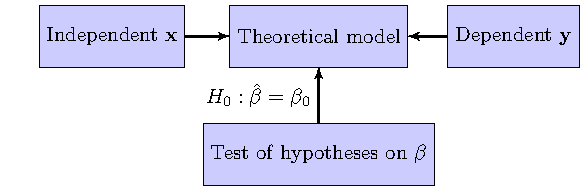
\includegraphics[width=0.49\textwidth]{./figures/modelapproach}
	}
	\hfill
	\subfloat[Data driven approach\label{dataapproach}]{%
		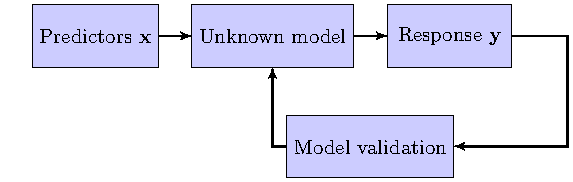
\includegraphics[width=0.49\textwidth]{./figures/dataapproach}
	}
	\caption{Two cultures of statistical/econometric modeling \citep[inspired by][]{breiman2001statistical}}
	\label{fig:twocultures}
\end{figure*}

Figure \ref{fig:twocultures} is an adaptation from the one displayed in
\citet{breiman2001statistical} and describes the processes governing these two
cultures. Figure (\ref{modelapproach}) is what I refer to as the modeling
approach, where a statistical model is postulated and is central to this
culture. This is the classical approach\footnote{Sometimes as well referred to
  as the frequentists' approach. However, this typically concerns the debate
  between classical statistics and Bayesian statistics, where the two approaches
  I refer to are more concerned with wider frameworks, of which the Bayesian
  approach is just one of the elements. I come back to Bayesian statistics and
  the frequentists' approach later, but I do not see them necessarily as
  opposites. And I quite object to the term frequentists' approach as Bayesian
  statistics is much more focuses on counting then the frequentists' approach.}
  where statistical probability theory
  meets the empiricism of Karl Popper.\footnote{To be honest, Popper himself was not a
  great fan of simply null hypothesis testing. He actually argued for the
  falsification of explanatory models, where in his view falsification does not
  only rely on statistics but on consensus amongst scientists as well.} Usually the model assumed is stated as a linear model and in its most simple form can be denoted as:
\begin{equation}
	\mathbf{y} = \mathbf{x}\beta + \epsilon, 
\end{equation}
where in (regional) economics language, $\mathbf{x}$ is referred to as the
independent variable, $\mathbf{y}$ as the dependent variable and $\epsilon$ as a
residual term. In this setup, using the data at hand, one constructs a
statistical test to which extent the estimated coefficient (denoted with
$\hat{\beta}$) deviates from a hypothesized value of the coefficient (denoted
with $\beta_0$)---typically the hypothesis $H_0: \hat{\beta} = 0$ is used with
as alternative hypothesis that $H_1: \hat{\beta} \neq 0$. However, that is
always within the context of the \textit{postulated} model. So, when the
null-hypothesis is rejected, it not necessarily means that the true $\beta$ is
unequal to zero, it might also be caused by errors in measuring $\bf{x}$ or even
using the wrong \textit{model}!\footnote{One of the assumptions for regression
  techniques such as the one used here is actually no misspecification of the
  model, but---apart from some possible tests on the functional form
  \textit{within} a specific regression form---usually little attention is give
  on the validity of the model used. More importantly, within this framework the
  model itself is usually not tested \textit{a posteriori}.}\footnote{There is
  another fallacy with this approach that is often overlooked and that is that
  the alternative hypothesis being true is a probability as well. Namely,
most hypotheses researchers test are typically not very probable. Not taken this
into account would actually lead to more null hypotheses to be rejected then
should be (false positives).}

Figure (\ref{dataapproach}) yields a schematic overview of a more data driven
approach. Here, we see an unknown model fed by predictors $\mathbf{x}$ that lead
to one or multiple reponses $\mathbf{y}$. The main objective here is not to test
hypotheses, but to find the best model instead which able to explain the
\emph{in-sample} data and to predict the \emph{out-of-sample} data.
Usually, the models are evaluated by some kind of criterion (e.g., the mean squared
error), which is not completely unlike the modeling approach. However, there are
two main differences between the two approaches. First, the data driven approach
considers several models in a structural approach. For instance, the question
which variables to include is captured by an exhaustive sourse of all
combinations in the modeling approach (e.g., with classification and regression
trees or random forests), while in the theory driven approach, the choice of
variables is based on the theory and a small number of variations in the
specification. Second, measurements on model performance are done
\textbf{out-of-sample} in the data driven approach and, typically,
\textbf{in-sample} in the model approach. The latter is not that important for
hypothesis testing, but for prediction this matters enormously, because adding
parameters might increase the in-sample fit, but actually worsen the
out-of-sample fit (a phenomenon called overfitting).  

In economics in general, and in regional economics
in specific, most of the tools employed are very much \textit{theory or model
  driven} instead of data driven. My (conservative) estimate would be that at least 90\%
of all empirical work in regional economics revolves around postulating a
(linear) model and testing whether (a) key determinant(s) is (are) significantly
different from a hypothesized value---usually zero.\footnote{In a seminal
  contribution, \cite{breiman2001statistical} states that deep into the 90s 98\%
  of the statisticians actually employed the theory driven paradigm and only 2\%
  a data driven paradigm. With the advent of the availability of internet
  connectivity, large (online) data sources, and faster computers the
  statistical realm changed dramatically. However, this has not permeated yet in
  the social sciences \citep[see as well][]{varian2014big}.} That is, \textit{within} the context of the model assumed.

At best, this approach can be seen in a causal inference framework. If a
determinant (such as a policy in the context of regional economics) $x$ changes, does it
cause then a change in the output $y$ (most economists typically use some
welfare measure).\footnote{Most of this research actually intends to mimic a
  \textit{difference-in-difference} approach and gained enormous momentum with
  the textbook of \citet{angrist2008mostly}.} This approach thus provides a
rigid and useful approach to regional policy evaluation. If we implement policy
$x$, does welfare measure $y$ then improve? Note that this always considers a
\textit{marginal} change as $x$ is usually isolated from other (confounding) factors.

However, policy makers oftentimes have different questions for which they need
solutions. Usually, they revolve around questions starting with \textit{``What
  determines performance measure $A$?''}, \textit{``Which regions can we best
    invest in?''} or, more generally, \textit{``What
  works for my region?''}. These types of questions require a different approach
than the previous one. Namely, the former type requires an approach focused on \textbf{explaining} while the latter type requires an approach focused on \textbf{predicting}.

The remaining part of this position paper is structured as follows. Section
\ref{practices} gives an overview of current modeling practices and describes the `traditional'
inference based approach as well as some data-driven approaches that have been
used in the recent past (though by far not as often as the traditional methods).
Section \ref{agenda} sets out both a research and an education agenda as it
addresses how to bridge the gap between the daily practices of regional
economists and the demands of local policy makers. The final section shortly
summarizes the main points raised in this position paper.  

%------------------------------------------------

\section{Regional economists turning the blind eye\label{practices}}

Unmistakenly, in the recent decade the two major changes to economic empirical research in general
are the advent of increasingly larger data sources and the large increase in
computer power \citep[]{einav2014economics}. The methods that mosts economists
employ, however, have not changed. Linear regression or one of its close
relatives (such as logistic, poisson or negative binomial regression), preferably in a causal
framework, is still the most common tool. This also applies to regional
economists, who---although coming from a tradition to use various methods from
different disciplines---have increasingly used similar methods as in
``mainstream'' economics.

This focus on marginal effects and causality is
certainly very worthwhile and brought us many important insights. However, it is
also typically done within a very narrow framework and, below, I will lay out what we are missing both in
research and in our educational curricula, when our \emph{main} focus is on the
framework above and as advocated so much as in \citet{angrist2008mostly}.   

\subsection{The blind eye in research}

The traditional model of a (regional) economist looks as follows:
\begin{equation}
  \label{model_economist}
  y_i = \alpha + \beta x_i + \mathbf{z}_i\gamma + \epsilon_i,
\end{equation}
where $y_i$ is referred to as the dependent variable, $x_i$ is the main variable of
interest, and $\mathbf{z}$ is a vector of other variables. $\alpha$, $\beta$ and
$\gamma$ are parameters, where we are especially interested in the value of
$\beta$. Finally, $\epsilon_i$ is an identical and independent distributed error
term.

Usually the main aim is to estimate $\beta$ as unbiased as possible in a causal framework. So, ideally, we
would like to control for unobserved heterogeneity bias, specification bias,
measurement error, reverse causality, selection bias, and so forth. Econometric
theory has produced some very powerful techniques to control for some of these
biases, such as instrumental variables, diff-in-diff procedures and the use of
fixed effects. However, these methods are not panacea for everything. First, they work
wonders for only specific research questions that have to do with the preferably
causal effects of marginal changes. Second, some of these techniques require very specific and
strong assumptions which are possibly not always met, which leaves doubts upon
the validity of the results. 

Below, I will deal with instrumental variables, diff-in-diff and fixed effect
techniques consecutively. I will specificially focus on some of the disadvantages. Some of the
arguments are adaptions from \citet{deaton2010instruments} and I refer to this
reference for a more complete treatise on the disadvantages of using
instrumental variables and diff-in-diff methods. For all the advantages not
dealt with in this paper, read \citet{angrist2008mostly}. 

\subsubsection{Exogeneity versus independence}

Economists love instrumental variables, because a good instrumental variable can
tackle reverse causality, measurement error and unobserved heterogeneity bias
all at one. Originally, instrumental variables come from simultaneous economic
models such as supply and demand models. A classical example in a regional
context would be:
\begin{align}
  P_r &=  \alpha + \beta E_r + \mathbf{z}_r\gamma + \epsilon_r, \label{P}\\
  E_r &=  \delta + \kappa P_r+ \mathbf{w}_r\lambda + \nu_r,\label{E}
\end{align}
where $P$ denotes population, $E$ employment and $z$ and $w$ are vector of other
regional $r$ characteristics. $\alpha$, $\beta$, $\gamma$, $\delta$, $\kappa$
and $\lambda$ are parameters to be estimated.

Obviously, one can not directly estimate (\ref{P}) and (\ref{E}) because of the
intrinsic simultaneity. However, suppose one is interested in estimating the
impact of employment on population growth, then one can use (\ref{E}) and search
for \emph{exogeneous}\footnote{This is not really precise; I mean exogeneous to
  population variation. I will come back to the use of exogeneous later.} variation in employment to use it as an instrumental
variable. A possible strategy could be to look into the population changes of
surrounding regions (but within commuting distance), as they might not have an
impact of the population change in the current region
\citep[see][]{DeGraaff2012, Graaff2012}

The main point\footnote{Directly from \cite{deaton2010instruments}.},
however, is that equations (\ref{P})--(\ref{E}) constitute a full-blown
economic \emph{model} which has direct relations with underlying structural
theoretical modeling frameworks \citep[such as][]{roback1982wages}. And the
instrument then comes directly (is interal) from the model. 

In practice, however, researchers often take another approach. And that is to
look for external instruments. Instruments that have no relation with a
structural (simultaneity) model. And there are is (a large) potential pitfall when doing so
and that is to end up with an instrumental variables that is not independent from
the left-hand-side variable. As it seems, there is some confusion about terms as
independence and exogeneity, so let's first clarify the exact assumptions a
valid instrument should satisfy.

Suppose that somebody is interested in the impact of population on employment; so, one would like to
identify $\kappa$ in (\ref{E}). To control for endogeneity researchers then
search for an \emph{exogenous} and \emph{relevant} instrument, $Z_r$. The latter
indicates that the instrument has an impact on the possible endogeneous variable
($P_r$) and the former indicates that the instrument does not affect the
left-hand-side variable ($E_r$), only via $P_r$ and other instruments. In formal
notation: $E_r \perp Z_r|P_r, w_r$. Thus, exogeneity means that the instrument
and the left-hand-side variables are \emph{independent} from each other conditional on
the instruments.

Unfortunately, exogeneity is often used as an argument for variables that are
external to the system, denote a sudden shock or for phenomena that are
considered to be exogenous in other fields (such as in geography).
And this usually leads to instruments that do not satisfy the
independence assumption. I will give three examples below.

First, and very often use is the concept of deeplagging. So, in our case, we
look for regional population say 100 years ago and use that as an instrument. It
must be exogenous because we cannot change it, right? Well, it is definitely
relevant, as regional population is remarkably resilient. Where people lived
100 years ago, they most likely live today. But, if we take model
(\ref{P})-(\ref{E}) seriously, then the population 100 years ago, must at least
have affected employment 100 years ago, and if population is resilient then most
likely employment as well (and we even do not consider yearly temporal dynamic
between population and employment). So, in all likeliness, employment and
population 100 years are not (conditionally) independent.

The second type of instruments people often use are regional characteristics
(preferably deeplagged as well), and specifically accessibility measures as
road, railroads and canals. For a large audience the following story typically seems very plausible at first
sight. At the end of the 19th century the large scale introduction of the
railways enabled households to live further from home and escape the heavilty
polluted inner cities where the factories remained (making use of the same
railroads intersecting in city centres). Railroads thus changed the location of
population and not that of employment. While this story is entirely possible,
what is often overlooked is the fact that factories and thus employment changed location as
well, but only 20-30 years later, and typically along the same links as opened
up by railway lines. So, the railway network 140 years ago and contemporary
location of employment are not (conditionally) independent.

A last often used category of candidate instruments is geography-related
variables. In our case that could be regions of municipalities. For instance,
the Netherlands witnessed for a large period intensive population location
policies. This entailed that the dutch government pointed out municipalities
that were allowed to grow (in terms of housing policies). Using fixed effects of
these specific municipalities then as instruments sound as a viable strategy.
However, this requires strict assumptions. Namely, being a specific municipality
will only have an effect on employment through being designated by the Dutch
government; and by nothing else.\footnote{A similar argument has been made by
  \cite{deaton2010instruments}, who considers economic growth theory, where fixed
  effects of specific countries are used as instruments because they took part
  in specific agreements---i.e., the Camp David accord for Egypt. Then the
  heroic assumptions has to be made that being Egypt has no effect on growth,
  except for the Camp David accord.}

Is this to say that instrumental variables is a bad technique? No, absolutely
not. If the instrument is valid, this is one of the most powerful techniques in
the econometric toolbox. The point made here is that good instruments are
actually hard to find and that structural simultaneous models (typically, in the
context of supply and demand) usually work better to find instruments than
instruments that are completely external to your problem. And if you really need
to use an external instrument, be very specific and open about the assumptions
you need to make.

\subsubsection{Local and average treatment effects}

Two concepts which have received quite some attention recently in econometrics, but is often
overlooked in applied regional and urban economics are local average treatment
effects and average treatment effects. The former deals with the interpretation
of instrumental variables, the latter with the (interpretation) of spatial
difference-in-difference methods. Even though those methods are different, they
have similar consequences for the interpretation of research findings and their
unlying assumptions.

The \emph{Local Average Treatment Effect} (or the LATE theorem) deals with the underlying
assumptions that have to be made so that the instrumental variable estimation
actually measures what we want \citep[see][]{imbens1994identification}. Referring again to our example above and say
that we want to instrument regional population changes with municipalities being
designated by a national policy to increase local housing supply. What we then
actually measure is the effect of changes in population on employment of those
municipalities that have actually complied with the national policy.
Municipalities that dropped out in an earlier stage are not taken into account,
but municipalities who did comply but never implemented the policy are.

So, what is actually measured is the designation of municipalties to a policy,
which might be a very interesting research question indeed, but in all
likelihood does not necessarily coincide with the coefficient $\kappa$ in
model (\ref{E}) above. In almost all cases the LATE theorem points at a more
restrictive effect (and thus interpretation) of the instrumental variable than
the \emph{structural} model sets out to estimate. Only under very strong
assumptions---homogeneity of regions, perfect compliance, and so forth---
the coefficient by the instrumental variable coincides with the coefficient of
the structural model.  

A different but related issue is that of the average treatment effects. Since
the seminal work of \citet{angrist2008mostly} difference-in-difference methods
(and all its variants) gained enormously in popularity. As well as in regional
economics where spatial difference-in-difference are applied as often as
possible. The idea itself is rather straightforward and originates from the
search for semi-experimental randomized controlled trials (RCT's). 

For the regional domain, assume the following: there is one group of
municipalities that implement a policy (the treatment; $T = 1$) and one group of municipalities that does
not ($T = 0$). Both groups of municipalities are measured before ($t = 0$) and after
implementation ($t=1$).
Then we can rewrite model (\ref{model_economist}) as:

\begin{equation}
  \label{eq:diff}
  y_r = \alpha + \gamma_1 T_r + \gamma_2 t_r+ \beta (T_r \times t_r) + \epsilon_r,  
\end{equation}
where $Y_r$ denotes a specific regional outcome variable, $T_r$ the set of
regions that are treated and $t_r$ the post implementation period. In this
set-up $\gamma_1$ measures the average impact of the treated regions, $\gamma_2$
the impact of the time period, and $\beta$ is our coefficient of interest; being
the impact of the treatment. Note that $\beta$ in this setting actually denotes
the difference in the outcome of the treatment groups \emph{minus} the
difference in the outcome of the non-treated groups: hence, the name
differences-in-differences.

The main assumption for this technique relies on the trueness of randomization of treatment
across, in our case, municipalities. In reality, the concept of randomization is
difficult to defend. Poor regions are more likely to receive governmental
subsidies, accessibility improvement are usually implemented in dynamic and
succesful regions, and so forth. To circumvent this, researchers look at borders
between regions. Back to our example, we then look at individuals close to a
border between two municipalities, where one municipality received a treatment
and the other did not. It is then defendable that such a band around a border is
relatively homogeneous in characteristics an that both regions are thus equal
except for the receivement of treatment.  

This approach has two main consequences. The most mentioned consequence is that
the effect $\beta$ is a so-called mean treatment effect. Every region, firm or
individual benefits (is harmed by) equally from the treatment. So, it might very
well be that some regions benefit greatly from some a policy, while it is
actually harmful for others. Making the treatment effect more heterogenous is
difficult and requires a lot from the data as every subgroup needs its own
semi-experimental randomized control trial.

Extending this argument to spatial difference-in-difference methods leaves us
even with the assumption that the whole region should be alike the border area
in term of benefitting from the policy. Or one should be satisfied with the fact
that $\beta$ only tells us something about the effect of the policy in a border
area. An area most likely not very representative of the rest of the region. 

The other consequence relates again to the compliance assumption. Regions and
municipalities themselves can be argued to fit well in treatment or
non-treatment groups. And if not, non-compliance should be easily detected.
However, for firms and individuals, compliance to randomization
of treatment is often a very harsh assumption. More and more, evidence is found
that especially individuals are very resourceful to circumvent randomization,
whether it by allocation to class sizes, elementary schools, or even military
draft by lottery.

Randomized controlled trials and difference-in-difference methods are strong
techniques for the applied regional economist. The point here is, however, that
without very strong assumptions, findings are mean effects that only applied to
a limited part of total sample. 

\subsubsection{Fixed effects and heterogeneity}

An often used technique in applied econometrics is the use of fixed effects.
They work brilliantly in removing unobserved heterogeneity but they come at a
price which is typically overlooked. Namely, they remove valuable variation as well in
both the dependent (predictor) $x$ and the independent (reponse) variable $y$.

Consider the following model in equation (\ref{eq:density}), which is at the moment a heavily
researched issue in both regional and urban economics. The issue here is to what
extent city density increases individual productivity.  

\begin{equation}
  \label{eq:density}
  \ln(w_{ic}) = \alpha + \beta \ln(d_{ic})+\epsilon_{ic},
\end{equation}
$w_{ic}$ denotes here individual wages (as a proxy for productivity) and
$d_{ic}$ density of the city $c$ individual $i$ lives in. $\beta$ is our
parameter of interest and because of the log-log structure $\beta$ denotes an
elasticity. Obviously, direct
estimation of model (\ref{eq:density}), would lead to a misleading parameter
$\beta$ if one is aiming to measure a causal effect.\footnote{I specifically do not use
the term \emph{biased} here. Namely, model (\ref{eq:density}) is a perfectly fine
model to measure the overall correlation ($\beta$) between city density and individual
wages and mosts non-economists are perfectly fine with this model
\citep[see, e.g.,][]{bettencourt2010unified}. So, whether a parameter is biased depends ultimately upon the research question.}
Namely, $\beta$ might be influenced by other (confounding) factors than only city density. One
can think of factors such as skill level of the city population, accessibility of the city,
sector structure of the city and city government. Moreover, a phenomenon called
sorting might occur, where more ambitious, risk-seeking and high-skilled people
migrate into larger and more dynamic cities.\footnote{Another issue we will not
  deal with here is reverse causality where it might be that higher wages lead
  to larger in-migration and thus larger density. This can, however, not be solved
with fixed effects, but with tools as instrumental variables instead. We
therefore leave it out of the discussion in this paragraph.}

To answer the question to what extent density causes wages, researchers
therefore resolved to using fixed effects. A baseline model can be seen in
(\ref{eq:fe}). 

\begin{equation}
  \label{eq:fe}
  \ln(w_{ic}) = \nu_i + \xi_c + \beta \ln(d_{ic})+\epsilon_{ic},
\end{equation}
here, $\nu_i$ denotes individual $i$ specific fixed effects and $\xi_c$ city $c$
specific fixed effects. So, everything that does not vary over time for
individuals and cities is now controlled for. A more insightful way what exactly
happens is to write model (\ref{eq:fe}) in changes, such as: $\Delta \ln(w_{ic}) =
\beta \Delta\ln( d_{ic}) + \epsilon_{ic}$.\footnote{Using changes (first differences)
to remove fixed effects is a viable but often overlooked technique for dealing
with fixed effects.}. So our model (\ref{eq:fe}) now identifies the
\emph{causal} effect by looking at the impact of a change in density on a change
in wages \emph{for the same individual within the same city}.

Multiple improvement have already been to this model including controlling for
sector/task of work and migrating between cities. Including these fixed effects
(and many more) has had a profound effect on the value of $\beta$. Directly
estimating model (\ref{eq:density}) yields an elasticity of around $1.15$,
while estimating a model such as (\ref{eq:fe}) including many fixed effects
would yield an elasticity of around $1.02$. So, there are economies of
agglomeration, but they are not very large.

\begin{figure*}[t!]\centering 
	\subfloat[Fixed effects\label{fe}]{%
		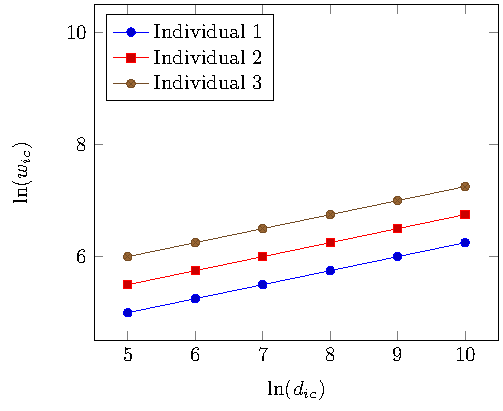
\includegraphics[width=0.49\textwidth]{./figures/fe}
	}
	\hfill
	\subfloat[Heterogeneity in $\beta$\label{heterogeneity}]{%
		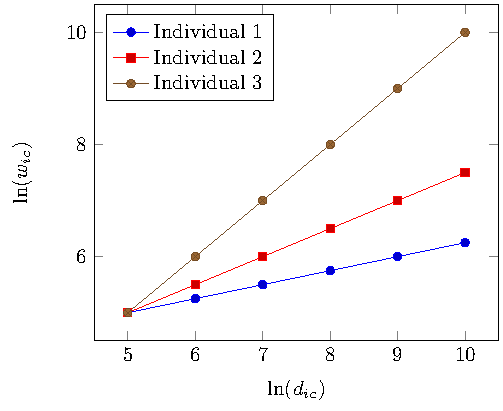
\includegraphics[width=0.49\textwidth]{./figures/hetero}
	}
	\caption{Heterogeneity in levels versus slopes.}
	\label{fig:heterogeneity}
\end{figure*}

Is this now the end of the story? Alas, it is not. At least three remarks can be
made which put the above into perspective.

First of all, note that we need changes over time---in our case in individual wages and
city density. Now, if we take the extreme example of a subgroup of individuals
who do not face wage changes and cities who remain relatively of equal size,
than this subgroups will not be used for determination of $\beta$. Of course,
not many observations will have these characteristics. Unfortunately, with
more detailed data on sector structure and migration, we need individuals that
move both residence and job for identification. All others are redundant. This
increases the risk on what is called sample selection bias---identification is
based on a specific subgroup with deviant characteristics. The point made here,
is that with the use of many fixed effects, much is demanded from the data and
one need always check whether the sample used for identification is not too
restrictive.  

Secondly, if there are unobserved factors that both relate to wages and density,
then it is actually very likely that these unobserved factors are related to
their \emph{changes} as well. One particular example here is technological
change, which might affect density (suburbs) and wages at the same time, and is
definitely not time-invariant. If one thinks about it, most interesting
socio-economic phenomena are not time-invariant, except perhaps longitude and
latitude. For example, a specific argument to use fixed effects is to control
for local attractivity. But what individuals and firms find attractive does
change of time, especially within cities, but across cities as well. Before
air-conditioning cities in Florida and Nevada were definitely not as popular as
today. And malaria-rich areas such as wetlands and river banks were always
avoided until recently.   

Thirdly, the use of fixed effects is based upon the assumption that all
variation is based on variation of \emph{levels}. That is, each fixed effects
actually denotes a very specific constant (for each individual and city in our
case). However, this really requires a very homogeneous sample except in levels.
For illustration, assume that there are three individuals, where individual 3
has gigher wages than individual 1 and 2, because of, say, differences in skill
levels (see as well Figure \ref{fe}). However, as Figure \ref{fe} clearly shows
as well, apart from individual level variation, returns to density are similar
for individuals 1, 2 and 3. So, each individual benefits equally from moving
from a small village not a large metropolitan area. Now, assume that individuals
are different with respect to the returns by living in large and denser cities.
Then the impact $\beta$ should also differ amongst individuals as is illustrated
in Figure \ref{heterogeneity}. This is not an argument to say that using fixed
effects is wrong. But if the sample might be heterogenous, i.e. that
units respond differently to different predictors, then using fixed effect might
not yield a complete pictures and in some specific cases even a distorted picture. 

Fixed effect techniques is a must have for every empirical regional economists.
However, the message I would like to convey here is that it does not remove
time-invariant unobserved heterogeneity (of which there is more than most
researchers realise), is not very suitable for tackling heterogeneity in your
main effect and might lead in some cases to sample selection bias.

\subsection{The blind eye in education}

So, if the main instruments of regional economists are not always applicable and
we miss tools in our toolbox to tackle, e.g., heterogeneity, prediction and
non-marginal changes, how do we then fare in teaching? Are the students who now
graduate equipped with the right toolbox that they use as well in their later
careers? And do we have a consistent curriculum using similar or complementary
tools running from the bachelor to the graduate studies? These types of
questions are not frequently asked, and, if at all, not very well met. Mostly
because of vested interests of departments and researchers.

In this subsection I will, however, try to answer partly some of these questions
and identify what is missing in our curriculum. I will first look at the
traditional applied econometrics approach and then to the (non-existence) of
other courses geared towards data science, including the use of statistical software.

\subsubsection{Statistics \& Applied Econometrics}

In contemporary economic bachelor curriculae students typically follow one
applied statistics course, where some hands-on experience is offered by working
with small datasets---typically in menu driven statistical software such as SPSS
or STATA. In the master phase, if students start to specialise in, e.g.,
regional economics, students then follow one applied econometrics
course with an emphasis on regression techniques, instrumental variables and the
use of fixed effects.

The statistics courses are very much geared towards traditional socio-economic
research where a hypothesis is formed (usually the difference between two groups
not being zero), data is gather (via survey techniques) and statistical tests
are applied on the difference between two groups (usually with the use of
$t$-tests).

For most students, especially applied statistics feel as a very mechinal
procedure using a pre-defined set or recipes. \citet{mcelreath2016statistical}
introduced a nice analogy with the old folkore of the Golem of Prague. The
Golem was a mindless robot of clay that obeys orders. Scientists also use
golems, especially with statistical procedure, where test or estimation one
performs is a small golem in itself. A mindless procedure that obeys what you
tell them do. Sometimes for the better, sometimes for the worse. 

For students this is not completely unlike: if you have this procedure, with
these data, you should use this test---if not, use that test. Why that test is
not an issue, one just follows a particular scheme and deploys one's own golem. What is
problematic with this approach is that students never completely understand what
they are doing. Throughout their bachelor years, the relation between test
statistics, $p$-values, significance level and confidence levels is typically
lost on them.

For a large part, confusion amongst students is caused by the fact that
(classical) statistics at the bachelor level is in way rather counter intuitive.
Take, e.g., the following two statements about the 95\% confidence interval.

\begin{quotation}
  A 95\% confidence interval means that for a given realized interval there is a 95\% probability that the population parameter lies within the interval.
\end{quotation}

\begin{quotation}
  With numerous repeated samples, the fraction of calculated confidence intervals (which would differ for each sample) that encompass the true population parameter would tend toward 95\%.
\end{quotation}

Most students---in fact the audience at large and most scholars as well---would
choose the first statement as being true for the 95\% confidence interval. But
in fact, the first statement is wrong and the second is true. The confidence
interval is only formed by the (often implicit) assumption of numerours (infite)
sampling. It does not resemble a statement about a probability of the population
parameter even though most us feel intuitively that that \emph{should} be the
case.

These concepts of sampling and the associated confusion unfortunately,
carry directly over to the applied econometrics domain. However, usually
students find applied econometrics easier as less emphasis is put on the
statistical background of the estimators. Unfortunately, applied econometrics
only comes back in non-methods courses in the master phase, less so in the bachelor years,
even though concepts as regression is taught in the first bachelor. This
typically leaves bachelor students with a small amount of experience and less to none
intuition when it comes to applied (econometric) work with empirical datasets.   

as I will argue in the next section there are other ways of teaching students
concepts of statistics and probabilities which rely less on sampling and more on
counting (frequentism) instead. However, for this, computers and statistical
software packages are needed, but then at least we can make statement as the
first one above, which feel far more intuitive. 

\subsubsection{The usage of data science}

In addition to statistics and applied econometrics, students are now offered a
(data science) programming language as well in the
bachelor, mostly R of Python. They usually only learn the basics and typically
do not work with databases, datascience of modeling techniques in these type of
courses. And, unfortunately, subsequent bachelor courses do not use these programming
languages for their exercises. This renders the added value of these courses
quickly to zero.

Master courses now use more and more data science techniques and languages,
although---in all honesty---typically outside the domain of (regional)
economics. Unfortunately, without a solid background in dealing with data
management and newer and more applied concepts of statistics, students approach these forms of
techniques (e.g., classification and regression trees) again as mechanical
golems by following recipes without truly understanding the underlying theory.   

%------------------------------------------------

\section{Incorporating the data science culture\label{agenda}}

The previous section discussed contemporay and cutting-edge methods of (regional)
economists. As argued, these methods have merits. Not least because they are all
geared towards identifying \emph{causal} relationships, and to a far greater
extent then in other social sciences.

However, these methods do come at some costs. First of all, the results should
be interpreted as \emph{marginal} effects. A small change in $x$ causes a
certain change in $y$. Second, the effect is always \emph{ceteris paribus}.
All possible other factors are controlled for. Third, most of these methods face
difficulties with \emph{heterogeneous} effects. Fourth, and final, the underlying
statistical framework is often difficult to interpret---for students, scholars,
and the audience at large.

These disadvantages do have serious consequences for what this traditional
toolkit can and what it cannot. First of all, it is very
good in explaining but very bad in predicting. Second, system-wide changes and
impacts are difficult to incorporate. Third, it has difficulties with different
heterogeneous subgroups. Fourth, the underlying statistical framework makes it
difficult to evaluate models. And, as last, the statistical framework also make
it difficult to deal with non-linear and non-parametric techniques are
difficult to yield with this specifications.

Below, I first explain how using techniques from the data driven approach side, or the
data science side, can help research in  the field of regional economics further in three
directions: model comparison, heterogeneous effect sizes, and predicting.

Thereafter, I describe what needs to be changed in education, so that future
students will better enabled to deal with the abundance of larger datasets, the
need for better predictions and a more intuitive understanding of probabilities
and testing.

\subsection{In research}

\subsubsection{Dealing with heterogeneity}

One of the weaknesses of the theory driven approach---or the more classical
research methods---is dealing with heterogeneity. Fixed effects regressions
only deal with removing level effects and not varying slope effects,
difference-in-difference designs only give average treatment effects and
instrumental variables have difficulties with incorporating
heterogeneity\footnote{There are some advances made in introducing
  heterogeneous instuments in quantile regression techniques, but the exact
  mechanism is still not clear-cut.}.

The argument made against heterogeneity is that it only affects efficiency
(i.a., the standard errors), but in most cases this is not true. In non-linear
models, such as discrete choice and duration models heterogeneity affects the
consistency (i.a., the parameter of interest) as well. Moreover, interpration of
the parameter of interest might be completely off when not allowing for
heterogeneous groups. 

\begin{figure*}[t!]\centering 
		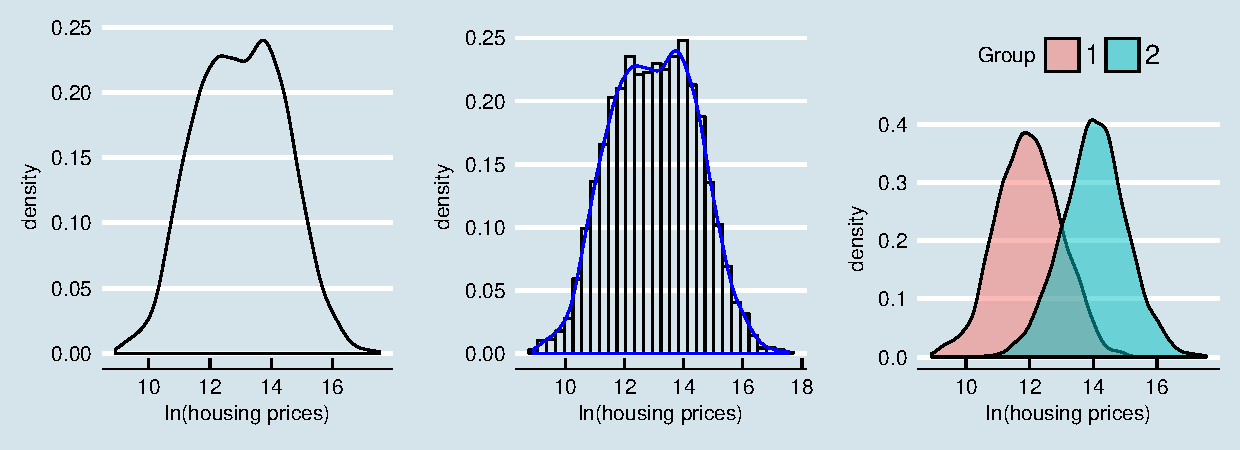
\includegraphics[width=\textwidth]{./figures/mixture}
	\caption{A mixture of two distributions of housing prices.}
	\label{fig:mixturetwocultures}
\end{figure*}

Consider Figure \ref{fig:mixturetwocultures} where in the left panel a density
distibution is given from a distribution of lognormally distributed housing
prices. When interested in explaining the effect of a variable $x$ on housing prices
this is typically the first descriptive plot an applied researcher creates. The
middle panel enlights this plot further by combining both a density plot and a
histogram. But what if the sample consists of \emph{two} types of housing
markets. One overheated and one with ample housing supply. Then most likely the
mechanism on both markets are different and the effect $\beta$ could be very
well different for both markets. Indeed, the right panel shows that the density
distribution from the left panel is actually a realization of a mixture of two
(in this case normal) distributions. The housing market with ample supply of
houses is then represented by group 1 and the overheated housing market is
represented by group 2.

These latent class approaches are typically not much applied in (regional)
economics \citep[see for an exception, e.g.,]{lankhuizen2015}.\footnote{In other
ecoomic or social science fields, such as market and transportation science,
however, this is already a common approach.} However, correct identification of
submarkets or subgroups could be very important for policy makers as the average
treatment effect may very well not even apply to anyone \citep[an argument, in
Dutch, made as well in][]{DeGraaff2014misc}.  

Slowly, the notation that fixed effects contain much useful information
permeated in the regional economics domain. An insightful and straightforward
way to do this is by adapting the wage model in (\ref{eq:fe}) as follows:
\begin{align}
  \label{eq:fe2}
  \ln(w_{ic}) &= \xi_c + \beta \ln(d_{ic})+\mathbf{z_{ic}}\gamma + \epsilon_{ic} \notag \\
  \xi_c&=\alpha + \mathbf{x_c}\delta + \mu_c,
\end{align}
where the individual wage model is now split up in two stages. The first stage
model the individual variation and regional fixed effects. The second stage now
regresses regional variables on the estimated fixed effects. This approach is
now frequently applied \citep[For example, in the so-called sorting
model][]{Bayer2004, Bayer2007a, Wang2016,
  Bernasco2016}. 

Two large advantages of this approach are that the standard errors on both the
individual and the regional level are correctly estimated and that, if needed,
instrumental variable methods may be applied in the second stage. There is one
disadvantage and that is the fixed effects in the second stage are not observed
but estimated (imputed) and that has an effect on the standard errors.

Note that model (\ref{eq:fe2}) is very much alike multi-level models, which are
very often used both in the data driven approach and in other social science
apart from economics. Multi-level modeling works great in both correctly
estimating a model with observations on various levels (such as individuals, firms,
sectors and regions) and in retrieving heterogeneous estimates (both in levels
and in slopes). Unfortunately, correcting for possible endogeneity is cumbersome
in multi-level modeling. But, with the increasing advent of micro-data,
combining a individual-regional model as in (\ref{eq:fe2}) with the more
rigorous structure of multi-level modeling is definitely worth more attention in
the near future. 

Interestingly, more (spatial) non-parametric approaches \citep[see, e.g., the
geograpically weighted regression exercise in][]{Thissen2016} have become more
popular as well in the last decade (typically, because of increased computer
power). This approach needs more attention as well, as the connection with
(economic) theory is often lost. And, especially regional geographers apply
spatial non-parametric techniques, not the regional economists 

\subsubsection{Model comparison}

One element that is notoriously weak in the theory-driven approach is model
comparison---or the models should be nested. And in many cases, model comparison
is often very much asked by policy makers and the audience at large, if not only
for finding the correct specification. The latter question is concerned with the
question which variables (predictors) to include in a model and which predictors
of them perform best. Note that this is analogous to questions regional policy makers
might have: such as, which policy instruments best to deploy given limited
financial budgets.

A typical example can be found in the field of spatial econometrics model where comparison is an important
issue as typically there are several competing theories, non-nested, for the
distance decay function (usually measured with a so-called spatial weight matrix
$\mathbf{W}$). And usually those theories are very much related (e.g., distance
decay measured in Eucledian distance or generalized travel costs).

Another field where model comparison is of large importance is in the estimation
of the strength of socio-ecoomic networks. In theory, socio-economic networks
should produce so-called power-laws: or a loglinear relation between the size of
nodes and the number of connections.\footnote{One of the most famous of these
  relations is Zipf's law, where the ordering of cities and the size of the
  population follows an almost perfect loglinear distribution; see for an
  in-depth treatment \citet{gabaix1999zipf}.} Empirically, these relations often follow a
slightly different distribution. What kind of distribution fits then best is
still a matter of debate.  

For proper model comparison, a Bayesian approach is almost unavoidable. The key
difference between the frequentist and the Bayesian approach is how to interpret
uncertainty. In the frequentist approach uncertainty originates from sampling,
while in the Bayesian approach uncertainty is caused by not having enough
information. So, a Bayesian statistian lives in a deterministic world but has
a limited observational view.\footnote{Both frequentists and bayesians rely
  heavily on sampling. However, sampling in frequentist statistics is a device to construct undercertainty
around an estimate. Sampling in Bayesian statistics is a way to perform integral
calculus (or to simulate observations).}. Note that the rule of Bayes is not
unique for Bayesian statistics. Namely, this rule is central for all probability
theory.

What is unique for each Bayesian model is that it has a prior and posterior. The
prior is an assumption about something that you do not know (uncertainty
measured by a parameter). With additional information (data), knowledge about
the uncertainty is then updated (and hopefully the uncertainty is diminished).
The updated probabilities are represented in a posterior distribution. To
understand the probabilities then is simply a matter of sampling from the
posterior distribution. So, the
frequentist approach typically give a point estimate of a parameter, the Bayesian approach
gives the whole distribution of the parameter. Note that under the Bayesian
paradigm , everything (including the data) is regarded as an variable with
associated uncertainty.

\begin{align}
  \ln(h_r) & \sim \text{Normal}(\mu_r, \sigma) \tag{likelihood}\\
  \mu_r & = \alpha + \beta x_r \tag{linear model}\\
  \alpha & \sim \text{Normal}(12,3) \tag{$\alpha$ prior}\\
  \beta & \sim \text{Normal}(5,10) \tag{$\beta$ prior}\\
  \sigma &\sim \text{Uniform}(0,2) \tag{$\sigma$ prior} 
  \label{eq:bayes}         
\end{align}
Model (\ref{eq:bayes}) gives an example of a Bayesian linear regression
model.\footnote{Under relatively mild assumptions this should yield similar
  results as the frequentist approach.}. Here, we want to model the relation
between regional housing prices ($h_r$) and the regional percentage of open
space ($o_c$). Note that all parameter and the distribition of the data
(likelihood) require distributional assumptions. This is a disadvantage in
relation to the inference based frequentist approach, where no distributional
assumptions are needed. But, note as well that model (\ref{eq:bayes}) specifies
\emph{explicitly} all assumptions for this model (e.g., a linear model and a
normal distribution for the likelihood). If you think the model is incorrect you
can rather easily change the assumptions.

Estimating Bayesian models have always been computionally cumbersome, especially
with more parameters as sampling from the posterior distribution equalizes
sampling from a multi-dimensional integral. Fortunately, computational power has
increased dramatically in the last decaded and techniques for sampling from the
posterior distribution have become rather efficient (the most often used
techniques nowadays are Monte Carlo Markov Chain algorithms which is basically a
simulation of the posterior distribution).

Although Bayesian statitics has already been applied to spatial
econometrics \citep[see the excellent textbook
of][]{lesage2009introduction}, applications have not permeated much to other fields
in regional economics, such as in regional growth estimations,
individual-regional multi-level modeling and population-employment modeling.  

\subsubsection{Predicting}

A last field not well developed in (regional) economics is that of predicting.
Most economists\footnote{In popular media, though, they are less hesitant to
  offer predictions.} would shy away from predictions as, in their opinion, identying
causal relations is already difficult enough (they have a point there). What
economists love to do is giving counterfactuals instead. For example, if
regional open space would decrease significantly, what would happens with
regional housing prices. This counterfactual approach looks very much as a
prediction, however there are two large disadvantages associated with
counterfactuals.

First, counterfactual are always made \emph{in sample}. Actually, all marginal
effects are made \emph{in-sample}. Splitting the sample in a training set and a
test set is not something that (regional) economists are prone to do. There is
an intrinsic worry then for \emph{overfitting}, especially when using many fixed
effects. Explanatory power may be very high, but could also be very situational
related. What works in one region, does not necessarily works in another region.
Note that predicting in spatial setting is more difficult as the unit of
analysis is typically a spatial system. And subsetting a spatial system in a
training and test set is often difficult.

Consider, e.g., the following often used gravity model in linear form as
depicted in (\ref{eq:gravity}): 
\begin{equation}
  \label{eq:gravity}
  \ln(c_{ij}) = \alpha + \beta \ln(P_i) + \gamma \ln(E_j) + \ln(d_{ij}) + \epsilon_{ij}.
\end{equation}
Here, we aim to model the number of commuters ($c$) from region $i$ to region
$j$, by looking at the total labor force $P_i$ in region $i$, the total number of
jobs $E_j$ in region $j$ and the distance ($d_{ij}$) between the two regions.
Suppose, we can improve the distance between region $i$ and $j$ by, e.g.,
enlarging highway capacity. This does not only change the commuter flow between
$i$ and $j$, but also between other region; say beween $i$ and $k$. As usual
there is no free lunch and total employment and population in each should remain
constant, at least in the short-run.

However, this make subsetting difficult and correctly predicting cumbersome.
But, model (\ref{eq:gravity}) of above is just one example of a large class of
models that all face this difficulty. And policy makers (and firms) are actually
very much interested in the questions associated with these predictions.
Questions related to the impact of Brexit on other countries, total network
effects of infrastructure improvements, identifying profitable routes for
airlines, impact of housing projects on commuting quickly come to mind. So, it
is especially the relation between predicting and spatial (interaction) systems
that need considerable attention.

A second problem with the counterfactual approach is that it considers marginal
changes. Unfortunately, in models as (\ref{eq:gravity}) this would not work. A
marginal change on the link between $i$ and $j$ would have marginal changes on
most other links. Marginal changes in a network setting is still a relatively
underdeveloped area.\footnote{That is, in applied empirical statistical work.
  Computational equilibrium models and to a lesser extent input-output models
  are able to model network-wide impacts. However, these models are cumbersome
  to construct and are less based on data.}

So, on of the main research challenges in the regional economic domain for the near future would be to combine
the data science models with the concept of spatial interaction models in such a
way that both predictions can be made and that model restrictions are still
satisfied. 

\subsection{In education}

In regional science in general and in regional economics in specific, remarkably little attention has been given to reproducibility and robustness of results \citep[with some exceptions as, amongst some others, by][]{Rey:2014cl,arribas2015woow, Arribas2016}.

\begin{figure}[t!]\centering 
  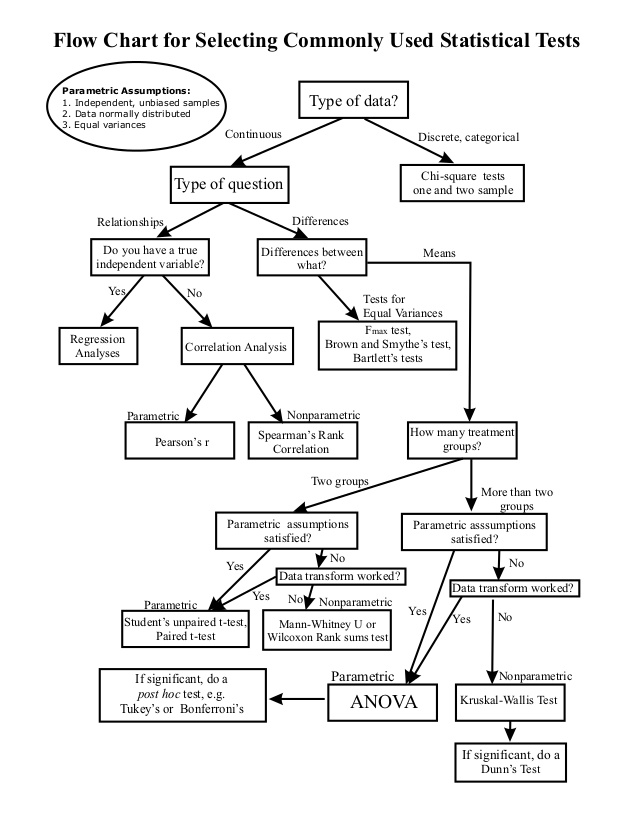
\includegraphics[width=\columnwidth]{./figures/flowchart.jpg}
  \caption{An example of a flowchart for statistical tests.}
	\label{fig:flowchart}
\end{figure}


\citet{schwabish2014economist}

\section{Into the abyss}

I started this paper with the observation, that, in the words of
\citet{breiman2001statistical}, there seems so be two cultures in statistical or
econometric modeling; a theory driven and a data driven approach. These two
approaches are not mutually exclusive, but complementary. And both have their
own strengths and weaknesses. However, especially in economics---and thus in
regional economics as well---the theory driven approach still seems to be highly
dominant, even with the advent of increasingly larger (micro-)databases.
Arguably, this is problematic as the theory driven approach has difficulties when anwering questions typically
asked by policy makers; questions such as ``What works best for my region?'',
``What happens with the capacity of my whole network when I invest in a specific
highway link?'' and ``In which region should I invest to get highest returns?''.

So, the main argument of this paper lies in introducing more data apprach/data
science techniques in the toolkit of the regional economist. Other related fields, even
in the social sciences, have already made large advances, such as predictive
policing in criminology, latent class approaches in transportion modeling, and
the use of deep learning techniques in marketing sciences. 

Obviously, this needs large investments (mostly in time), both for researchers
and for teachers. The first group needs to invest in new techniques and probably
in new statistical software. The second group needs to change parts of the
curriculum in terms of the specific contents of methods courses and exercises.
Fortunately, many online and open source manuals, videos and even textbooks are
available.\footnote{Especially for the R programming environment \citep{R2017}  there is a vast amount of
  material available on the internet, such as \href{http://r4ds.had.co.nz/}{R for Data Science}
  and \href{https://csgillespie.github.io/efficientR/}{Efficient R programming}.
Moreover, companies such as DataCamp allow for free subscriptions as long as the
material is used for classes.} 

To conclude, I would like to note that apart from the intrinsic scientific
arguments there are two other very compelling arguments to invest at least some
time in data driven approaches. First, it coincides wonderfully with other
techniques, such as versioning, blogging (publishing to HTML), and command line
tools. All these approaches ensure that research becomes more reproducible.
Something that becomes more and more a hard requirement by both university and
the audience at large. Second, when looking at recent advances both in industry
(e.g., all the dotcom companies but also others, such as more traditional media
companies) and in other scientific disciplines, it is not the question \emph{if} regional economists
should invest more in the data science approach, but the question \emph{how
  soon} can we start.  

%----------------------------------------------------------------------------------------
%	REFERENCE LIST
%----------------------------------------------------------------------------------------

\addcontentsline{toc}{section}{References} % Adds this section to the table of contents
\printbibliography

%----------------------------------------------------------------------------------------

\end{document}